\documentclass{article}

%\usepackage{epsfig}
\usepackage{tikz}
\usetikzlibrary{shapes,arrows,chains}

\usepackage[margin=0.75in]{geometry}
\usepackage[linesnumbered]{algorithm2e}
\usepackage{xcolor}
\usepackage{amsmath}
\usepackage{graphicx}
\usepackage{multicol}
\usepackage{wrapfig}
\usepackage{amsmath}
\usepackage{systeme}
\usepackage{enumitem}   
\title{SDSU COMP521 \\ Fall 2022}
\author{Homework 08 - Due Date: 12/09/2022}
\pagenumbering{gobble}
\date{}
\begin{document}
\newcommand{\norm}[1]{\left\lVert#1\right\rVert}
\maketitle

\section*{Problem 1}
The graph in figure \ref{fig001} shows the connection between four different web pages a, b, c and d. Rank the web pages using the approach based on the Perron-Frobenius eigenvector. Show the matrices used to solve the problem.

\begin{figure}[h]
	\centering
	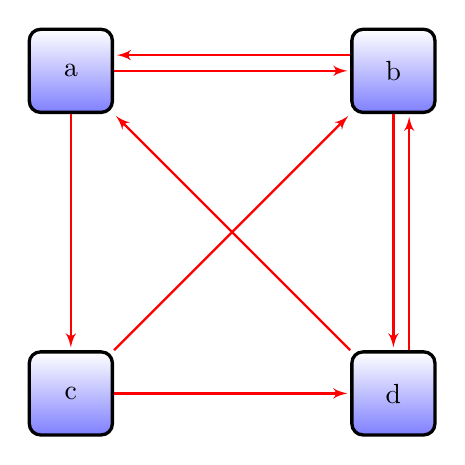
\begin{tikzpicture}[node distance=1cm, auto]  
	\tikzset{
		mynode/.style={rectangle,rounded corners,draw=black, top color=white, bottom color=blue!50,very thick, inner sep=1em, minimum size=3em, text centered},
		myarrow/.style={red,->, >=latex', shorten >=1pt, thick},
		mylabel/.style={text width=7em, text centered} 
	}  
	\node[mynode] (a) {a};  
	\node[mynode, right=3cm of a] (b) {b}; 
	\node[mynode, below=3cm of a] (c) {c};  
	\node[mynode, below=3cm of b] (d) {d};
	%\node[mylabel, below left=of a] (label1) {Participation rate $\theta_1$};  
	%\node[mylabel, below right=of a] (label2) {Participation rate $\theta_2$};
	% The text width of 7em forces the text to break into two lines. 
	
	\draw[myarrow] (a.south) --  (c.north);	
	\draw[myarrow] (a.east) --  (b.west);
	
	\draw[myarrow] ([shift={(0mm,2mm)}] b.west) -- ([shift={(0mm,2mm)}] a.east);	\draw[myarrow] (b.south) -- (d.north);
	
	\draw[myarrow] (c.east) -- (d.west);
	\draw[myarrow] (c) -- (b);
	
	\draw[myarrow] (d) -- (a);
	\draw[myarrow] ([shift={(2mm,0mm)}] d.north) -- ([shift={(2mm,0mm)}] b.south);
	% There is a slight overlap of the arrows with the (manufacturer) south edge
	% because creating the offset in another way didn't compile. 
	
%	\draw[<->, >=latex', shorten >=2pt, shorten <=2pt, bend right=45, thick, dashed] 
%	(c.south) to node[auto, swap] {Competition}(d.south); 
	% The swap command corrects the placement of the text.
	
	\end{tikzpicture}
	\caption{Links between four web pages}  \label{fig001}
\end{figure}

%\begin{figure}[h]
%	\centering
%	\includegraphics[scale=0.5]{HW8fig1.jpg}
%	\caption{Web sites graph}
%	\label{fig001}
%\end{figure}
%\begin{equation*}
%u_t + u_x = 0
%\end{equation*}
%where \\
%
%
%\begin{equation}
%u(x,0)=u_0(x) =
%\begin{cases}
%1 -|x|& \text{if $|x| < 1$ }\\
%0 & \text{otherwise}
%\end{cases}
%\end{equation}\\
%
%
%\textbf{Use Lax-Friedrichs} with space and time domains of $x \in [-2,10]$ and $t \in [0,8]$ respectively. Use left boundary condition $u(-2,t)=u_0 (-2-t)$ and right boundary condition $u(10,t)=u_0 (10-t)$. \textbf{Write your own code}.
%\begin{enumerate}
%	\item Show the plot of the numerical and exact solutions $u(x,t)$ at the first and last time points and three points inside the interval (your choice). Analyze and discuss the behavior.
%	\item Plot the error metric on a log-log plot for different values of $\Delta x$ you choose, at the final time step. Based on this plot, determine the order of spatial accuracy.
%\end{enumerate}

\section*{Problem 2 }
Choose an image of your preference and analyze it using PCA. Describe your work step by step and show figures/plots to support your results. You can do either an RGB or greyscale image.

%\begin{equation*}
%u_t + u_{xx} = 0 \quad  for \quad 0<x<1 \quad and \quad 0 \le t \le 0.1
%\end{equation*}
%
%, with the initial condition  $u(x,0)= f(x)= sin(\pi x)+ sin(3\pi x) \quad  \forall x \in [0,1]$ and boundary conditions:
%\begin{center}
%    $ u(0,t) = c_1 = 0 \quad for \quad x=0 \quad and \quad 0\le t \le 0.1 $ \\
%    $ u(1,t) = c_2 = 0 \quad for \quad x=1 \quad and \quad 0\le t \le 0.1 $ 
%\end{center}
%
%Solve the problem using the explicit scheme learned in class. Start with $\Delta x = 0.2$ and $\Delta t = 0.02$.
%
%\begin{enumerate}
%	\item Show the plot of the numerical and exact solutions $U$ and $u(x,t)$. You could use contour plots. Analyze and discuss the behavior. The exact solution is: 
%	$u(x,t) = sin(\pi x)e^{-\pi^2t} + sin(3\pi x)e^{-9\pi^2t} $
%	\item Plot the error metric on a log-log plot for different values of $\Delta x$ you choose, at the final time step. Based on this plot, determine the order of spatial accuracy.
%\end{enumerate}

%\pagebreak

%\section*{Problem 3 - Bonus Question for 5 points }
%We have the following PDE corresponding to the Laplacian equation:
%
%\begin{equation*}
%u_{xx} + u_{yy} = 0 \quad  for \quad 0 \le x \le 1 \quad and \quad 0 \le y \le 0.1
%\end{equation*}
%
%, where $u,x$ and $y$ are scaled variables and the following boundary conditions are imposed:
%\begin{center}
%	$ u(x,0) = 10  \quad and \quad u(x,1)=100 \quad for \quad 0 < x < 1 $ \\
%	$ u(0,y) = 50  \quad and \quad u(1,y)=0 \quad for \quad 0 < y < 1 $ 
%\end{center}
%
%Find the numerical solution using the finite difference scheme analyzed in class iteratively with Successive Overrelaxation (SOR).  
%Use  $\Delta x = \Delta y = h$  with $h=\{0.1 \,,0.01\,, 0.001\}$. Always set the same tolerance and maximum number of iterations at each $h$ used. Plot the numerical solutions using contour plots. Show a plot of number of iterations versus the problem size.\\



\section*{Deliverable}
You have to present a \textbf{REPORT} and submit it as a file in .PDF format. This report must describe the solution of each problem. It must describe and explain the results. Do not forget to identify the plots and tables. The report must present any script used.\\


\end{document}